                                                        
%\documentclass[sn-mathphys]{sn-jnl}
%\documentclass[compress]{sn-jnl}
\documentclass[sn-basic]{sn-jnl}
%\documentclass[sn-standardnature]{sn-jnl}
\jyear{2021}

\theoremstyle{thmstyleone}
\newtheorem{theorem}{Theorem}

\newtheorem{proposition}[theorem]{Proposition}%


\theoremstyle{thmstyletwo}
\newtheorem{example}{Example}
\newtheorem{remark}{Remark}

\theoremstyle{thmstylethree}
\newtheorem{definition}{Definition}

\raggedbottom

\usepackage{amsmath}
\usepackage{listings}
\usepackage{graphicx}
\usepackage{diagbox}
\usepackage{booktabs}
\usepackage{natbib}


\begin{document}

\title[Article Title]{PatchID: A Overfitting Patches Identification Method for Automated Program Repair}



\author[1,2]{\fnm{Xuan} \sur{Zhou}}\email{212050276@hdu.edu.cn}

\author*[1,2]{\fnm{Xingqi} \sur{Wang}}\email{xqwang@hdu.edu.cn}




\author[1,2]{\fnm{Dan} \sur{Wei}}\email{weiwd@hdu.edu.cn}


\author[1,2]{\fnm{Yanli} \sur{Shao}}\email{shaoyanli@hdu.edu.cn}



\affil*[1]{\orgdiv{School of Computer Science}, \orgname{Hangzhou Dianzi University}, \orgaddress{ \city{Hangzhou}, \postcode{310018}, \state{Zhejiang}, \country{China}}}

\affil[2]{\orgdiv{Key Laboratory of Discrete Industrial Internet of Things of Zhejiang Province},
	  \orgaddress{ \city{Hangzhou}, \postcode{310018}, \state{Zhejiang}, \country{China}}}



\abstract{The patch generated by automatic program repair (APR) needs to be verified. APR usually uses the test suite as the criterion for verifying the correctness of the patch. However, the test suite is unable to fully represent the oracle of the program, which causes APR to generat a large number of overfitting patches that not only fail to fix the original error, but also cause new errors. In order to reduce the number of overfitting patches generated by APR, this paper proposes an overfitting patches identification method for APR, PatchID. The core idea of PatchID is that the dynamic behavior of the passing tests between the buggy program and the correct patch is the same, however the dynamic behavior of the failing tests between themis different. The algorithm first constructs the dynamic behavior expressions that cause the bug from the program and the test suite, then generates new tests to enhance the original test suite, and finally gets the same dynamic behavior expressions from the patch, and identifies whether the patch is overfitting according to whether the value of the dynamic behavior expression changes with the use of the patch. The paper is evaluated on two datasets consisting of 157 Defects4J patches and 380 Java+JML patches, respectively. PatchID successfully identifies 63 overfitting patches and 15 correct patches on the first dataset, and 169 overfitting patches on the second dataset. In addition, PatchID classifies overfitting patches into three types of patches. Experiments show that the method proposed in this paper is superior to the existing similar methods.}


\keywords{automatic program repair, overfitting patch, program state abstract, test generation}



\maketitle
\section{Introduction}\label{sec1}

Automatic program repair (APR) has been widely studied in the past decade, and a large number of repair technologies have been proposed. Especially after the emergence of GenProg\citep{bib1}, the APR based on test suite occupies the vast majority. The test suite based APR takes a given test suite as oracle and generates patches that are considered correct if they passes the test suite. Accurally, the test suite is weak and can not fully represent the oracle of the program, which results in the existence of patches that pass all the tests but are still wrong, that is, overfitting patches. As a result, APR technology produces a large number of invalid patches. Current APR technologies are far from mature, and most of them will simply accept patches that pass the test suite. According to Xin \citeyearpar{bib5}, the majority of patches generated by GenProg, AE  and RSRepair are incorrect. More recent techniques try to find many other strategies (e.g., using human-written patches, repair templates and condition synthesis, bug-fixing instances  and forbidden modifications) for repair. However their  repair performance is still lower.

Due to the low performance of current APR techniques,  software developers have to verify a large amount of patches manually to filter out overfitting patches, which consumes too many resources.  Therefore, it has become an urgent problem to identify overfitting patches. If a patch passes the test suite and is considered the correct patch, then simply enhancing the test suite can reduce the number of overfitting patches. However, automatic test generation tools can only generate test inputs, and the appropriate test outputs still need to be determined manually. Even so, these approaches still fail to express a complete oracle. It is very difficult to have a complete oracle for a program, especially for large projects. Nilizadeh\citeyearpar{bib7} used a formal method (specification and verification), JML as correctness criterion to successfully describe a small  project. However facing the large project, such as Defects4J\citep{bib49}, JML fails. And it seems impossible to use JML to describe such a large project.

At present, it is already very helpful to identify whether a patch is overfitting or not because quickly identifying overfitting patches can improve the success rate  of APR technology. Furthermore, if there is technology to subdivide overfitting patches, it can speed bugs fixing. According to Yu \citeyearpar{bib4}, overfitting patches can be divided into the following three categories:

\begin{itemize}
	\item A-Overfitting Patch: The patch does not completely fix the incorrect behavior nor does it destroy the original correct behavior.
	\item B-Overfitting Patch: The patch that fixes the original incorrect behavior but destroys the original correct behavior, which is also called regression.
	\item AB-Overfitting Patch: The patch destroys the original correct behavior instead of fixing the incorrect behavior.
\end{itemize}

Because the test suite is not complete, it is far from sufficient to  use the consistency of the actual output of the program and the test output, that is to say, the current APR technology does not take full advantage of the test suite, only uses the input and the output of the test suite, and does not dig into the hidden information in the test suite. At present, different overfitting identification methods have been proposed. Among them, the strategy proposed by Xiong\citeyearpar{bib8} is the first technology to mine the deep behavior of test suites and programs. Through the ideas of TEST-SIM and PATCH-SIM, the identification rate of overfitting patch can reach 56$\%$. The experiment of Yang\citeyearpar{bib6} shows that patches can modify the behavior of the program. They try to use program invariants to describe the program behavior and observe the program oracle from another view. Inspired by this, we propose a new technique, PatchID, to solve the problem of patch overfitting.

The goal of PatchID is to determine the category of a patch by digging into the correct behavior of the program based on a given test suite. While patches are able to pass the test suite, the passing tests reflect the correct behavior of the program, and the failing test reflect the wrong behavior of the program. From this point of view, patches should maintain the correct behavior of the program and modify the wrong behavior of the program. We believe that there are specific relationships between variables in a correct program, which are reflected by their values at runtime, and these relationships are a manifestation of the correct behavior of the program. So PatchID identifies a patch based on the following two important observations, which are from the perspective of program runtime variables:

\begin{itemize}
	\item PATCH-SIM: After using the patch, the dynamic behavior of the program of the passing test (the specific relationship between variables, which is represented by a 5-tuple in this paper) is similar to that before, while the dynamic behavior of the program of the failing test is different.
	\item TEST-SIM: When two tests have the same dynamic behavior, the two tests belong to the same category, that is, they belong to either the passing test or the failing test.
\end{itemize}

Based on the above two points, this paper designs and implements PatchID, and verifies the method on a dataset consisting of 157 patches. These patches are generated by APR techniques based on Defects4J, including HDRepair, jGenprog\citep{bib65}, ACS\citep{bib66}, jKail\citep{bib67}, and Nopol\citep{bib40}.The method presented in this paper successfully identified 63 overfitting patches and 15 correct patches from 157 patches. In addition, PatchID further subdivides the 63 overfitting patches into three categories, which is not available in other technologies at present. We also verified on the dataset composed of 380 Java+JML patches, and successfully identified 169 patches.To sum up, the contributions of this paper are:
\begin{itemize}
	\item 5-tuple for computing program execution similarity is proposed.
	\item An overfitting patch identification and subdivision algorithm is designed for automatic patch generation.
	\item The framework of overfitting patch identification is implemented and the proposed method is evaluated. The results show that the proposed method is effective.
\end{itemize}

The rest of the paper is organized as follows. Section 2 begins with a discussion of related work. Section 3 describes some of the necessary concepts involved in the approach of this paper. Section 4 describes the method in this paper in detail. Section 5 presents an experimental evaluation of the method presented in this paper. Finally, the paper is summarized in Section 6.

\section{Related work}\label{sec2}
\textbf{Automatic Program Repair.} Generally, automatic program repair includes three steps: fault location, patch generation and patch verification. They will first generate some candidate patches, then use the existing test suite to verify these candidate patches, and the candidate patches that pass the test suite will be regarded as the correct patches. At present, the existing methods can be roughly divided into the following three categories:

\begin{itemize}
	\item Heuristic Search-Based APR: Heuristic search-based automatic repair technology generates the repair patch by artificially defined heuristic rules. This kind of algorithms inlcude GenProg, ARJA-e\citep{bib11,bib14}, PraPR\citep{bib9}, etc, which use genetic algorithm to generate patches with the original program as search space. In addition, there are approaches, such as HistoricalFix\citep{bib15}, CapGen\citep{bib16}, ConFix\citep{bib17} to generate patches from historical repair patches and those as SCRepair\citep{bib18}, CRSearcher\citep{bib19}, SSFix\citep{bib20}, SimFix\citep{bib21}, Refactory\citep{bib22} to generate patches bycode similarity.
	
	\item Template-Based APR: It generates patches based on manual template.  According to the experience of developers or researchers, some patch templates or patch generation strategies are predefined to guide the repair process. PAR\citep{bib74}, iFixR\citep{bib24}, SapFix\citep{bib25}, ErrDoc\citep{bib26}, BovInspector\citep{bib27}, LeakFix\citep{bib28}, AutoFix\citep{bib29}, GumTree\citep{bib30}, SketchFix\citep{bib31}, NPEfix\citep{bib32}, F1X\citep{bib33}, HERCULES\citep{bib34}, and the anti-pattern method proposed by Tan\citep{bib35} fall into this category of algorithms.
	\item Semantic Constraint-Based APR: Semantic Constraint-Based APR infers the correct specification of the program by some means as a constraint to guide the patch generation or to verify the correctness of the patch. SemFix\cite{bib36}, DirectFix\citep{bib37}, Angelix\citep{bib38}, AllRepair\citep{bib39}, Nopol\citep{bib40}, S3\citep{bib41}, SemGraft\citep{bib42}, MemFix\citep{bib43}, FootPatch\citep{bib44}, SearchRepair\citep{bib45}, SOSRepair\citep{bib46} belong to this kind of algorithms.
\end{itemize}

All these repair techniques use G$\And$V method to produce patches. For these technologies, if a patch passes the test suite, it is the correct patch. However, a program cannot be fully tested, and the test suites given by existing datasets are all weak\citep{bib10}, so repair techniques will always produce a large number of overfitting patches on these datasets. New techniques are needed to find to identify these overfitting patches.

\textbf{Patch identification.} Facing the problem of overfitting patches, researchers have proposed many methods. Xin\citeyearpar{bib5} identifys patches by generating new test inputs and checking semantic differences between buggy programs and patches. Nilizadeh\citeyearpar{bib7} uses JML as an oracle on small programs to verify the effectiveness of APR technology, but JML does not work while facing large projects like Defects4J. Xiong\citeyearpar{bib8} proposed PATCH-SIM and TEST-SIM. Their methods do not need oracle, classify the newly generated tests (test input) heuristically, and use the similarity of program execution paths to identify patches. It is too strict for the method using execution path similarity to identify overfitting patches. And it doe not further subdivide that overfitting patch. Inspired by the existing methods, this paper reinterprets PATCH-SIM and TEST-SIM by calculating the dynamic behavior expression of the program. It identifys patches heuristically, and further subdivides the overfitting patches.


\section{PRELIMINARIES}\label{sec3}
To identify whether a patch is overfitting, PatchID relies on the following basic concepts.
\subsection{Program State Abstraction}
In order to describe the dynamic behavior of a program at runtime, this paper introduces the concept of program state abstraction \citep{bib47,bib48}. Program state abstraction is composed of program variables, basic expressions, extended expressions, and boolean expressions.

\textbf{Variables.} During the execution of each test, the values of these program variables are added into the set $ M_{\ell}$. These program variables are derived from two types of data.
\begin{itemize}
  \item Exact values of numeric and boolean types
  \item Object identifier for a reference type expression
\end{itemize}

\textbf{Expressions.} In a program, reference types or numeric types can be monitored. These type of variables make up the basic expressions, which include 
(1) local variables (including parameters of $M_{bug}$) declared inside $M_{bug}$ (the method where the bug occurs), and these variables are visible at $\ell$; (2) attributes of the class to which the $M_{bug}$ belongs; (3)Any expression that can be evaluated at $\ell$, but expressions with side effects such as increment, decrement, assignment, and creation cannot be monitored. In this paper, we use $E_{\ell}$ to denote the set of all monitorable basic expressions at $\ell$ ($\ell$ denotes the unique identifier of each statement). For each reference type $r$ in the $E_{\ell}$, the following two forms form the extended expression, including: (1) $r.f()$, $f()$ is a no-argument function and returns a type that can be monitored at $\ell$. (2) When $r$ is this, the attributes of $r$ are monitorable at $\ell$. In this paper, we use $X_{\ell}$ to denote the set of all extended expressions that can be monitored.

In order to explain the expression in detail, Figure \ref{fig1} and Figure \ref{fig2} show the buggy program and its corresponding patch. The buggy program functions as follows: The duplicate method receives two ArrayLists $(list1,list2)$ and an int $n$. Its function is to copy $n$ elements from $list2$ to $list1$.However, this program has an obvious error, which ignores the case that $n$ is greater than the length of $list2$, When $n$ is greater than the number of elements of $list2$, the program will throw Index Out Of Bounds exception. $if$ statement is appended into the patch to avoid this error. $count$ in the first line of the buggy program, $list1$, $list2$, and $n$ in the arguments, are all basic expressions that can be monitored. At this point, the extended expressions for $\ell$ are $list1.size()$, $list2.size()$, and so on.


\begin{figure}[htbp]
	\centering
	\begin{minipage}[t]{1\textwidth}
		\centering
		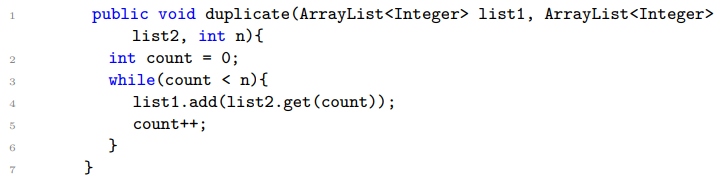
\includegraphics[width=1\textwidth]{fig1.png}
		\caption{Buggy program}\label{fig1}
		\vspace{5mm}
	\end{minipage}

    \begin{minipage}[t]{1\textwidth}
	\centering
	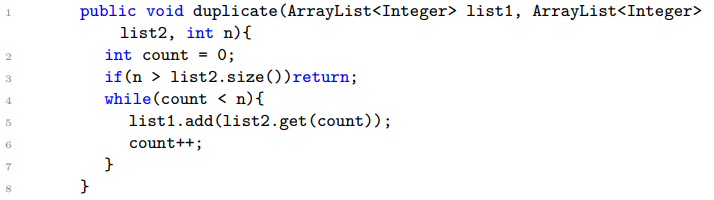
\includegraphics[width=1\textwidth]{fig2.png}
	\caption{Patch}\label{fig2}
	\vspace{5mm}
    \end{minipage}

	\begin{minipage}[t]{0.5\textwidth}
		\centering
		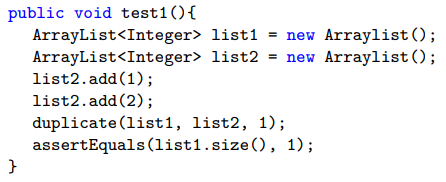
\includegraphics[width=1\textwidth]{fig3.png}
		\caption{Passing test: test1}\label{fig3}
	\end{minipage}
	\begin{minipage}[t]{0.48\textwidth}
		\centering
		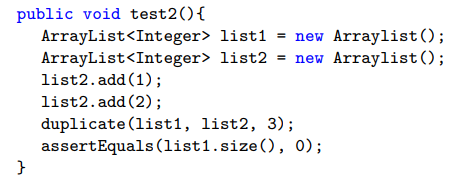
\includegraphics[width=1\textwidth]{fig4.png}
		\caption{Failing test: test2}\label{fig4}
	\end{minipage}
\end{figure}

\textbf{Boolean expressions.} Boolean expressions are composed of relational expressions and logical expressions. In this paper, we denote by $B_\ell$ a boolean abstract set at $\ell$. Boolean expressions can be expressed in the following four forms: (1)for each pair $k_1,k_2 \in E_\ell \cup X_\ell$ of expressions of the same type, $B_\ell$ includes $m_1 == m_2$ and $m_1 \neq m_2$; (2)for each pair $k1,k2 \in E_\ell \cup X_\ell$ of expressions of integer type, $B_\ell$ includes $k_1 \bowtie k_2$,for $ \bowtie \in \{ <,>,\leq,\ge \}$; (3)for each expression $b \in E_\ell \cup X_\ell$ of boolean type,$B_\ell$ includes $b$ and $!b$; (4)for each pair $b_1,b_2 \in E_\ell \cup X_\ell$ of expressions of boolean type, $B_\ell$ includes $b_1 \vee b_2$ and $b_1\wedge b_2$.

For example, in the first line of Figure \ref{fig1}, $n$ and $list2.size()$ are both monitorable expressions, and both are of the same Integer type. Then the following six boolean expressions can be composed:  $n>list2.size(), n>=list2.size(), n<list2.size(), n<=list2.size(), n==list2.size(), n!=list2.size()$.The boolean expression $n>list2.size()$ causes the program error. If the test satisfies this boolean expression, when the program enters the $while$ loop, $count$ will eventually equal $list2.size()$, which causes the program to throw an out-of-range error. So this results in test1 being a passing test and test2 being a failing test, because the size of $list2$ in test2 is less than 3.

\subsection{PATCH-SIM and TEST-SIM}
As mentioned earlier, a test suite is not like a formal specification in that its coding specifications are weak and incomplete. Low-quality test suites are a key reason why APR generates overfitting patches. To take full advantage of existing and enhanced test suites for filtering overfitting patches, we need the following two definitions:
\begin{definition}[TEST-SIM]
	When two tests have the same program behavior, then they will have the same test result, that is, the boolean expression b and the corresponding value are the same at the same statement, then both tests should be either a passing test or a failing test.  
\end{definition}
APR usually takes the patch that passes all tests as the correct patch, but the test suite cannot express a complete oracle. To enhance the test suite, we need to generate new tests, but PatchID's method of generating new tests does not and cannot know what the test output is. Only boolean expressions at run time are available. For example, there is a new test with $list1.size = 0$, $list 2.size = 5$, and $n = 10$. Then the boolean expression of the test in the third line of the buggy program in Figure~\ref{fig1} is $n > = list2.size(),true$, which is the same as the boolean expression of test2 at this point, so this test is considered to be a failing test.
\begin{definition}[PATCH-SIM.]
With the correct patch, the passing test is the same as the previous boolean expression and its value, while the failing test should be different. 
\end{definition}
For example, in a buggy program, all passing tests result in a boolean expression $b$ being false, and all failing tests result in $b$ being $true$.Then determining whether the patch is overfitting is not just a single way to observe the output of the program, but by comparing the value of $b$ in a statement before and after using the patch. The value of $b$ should be consistent with the buggy program when the patch runs the passing test; it should be different from the buggy program when the patch runs the failing test. According to PATCH-SIM, we can see that in the previous example, patch is correct, because in the fourth line (corresponding to the third line of the buggy program), $n > list 2.size()$ no longer exists, and all tests that make this boolean expression true will go to the $return$ statement.

Through these two observations, we can dig out more information from a buggy program and a test suite, so that the identification of patches does not need oracle. New tests are heuristically classified by TEST-SIM, and patches are heuristically classified by PATCH-SIM.

\section{APPROACH}\label{sec4}
This section mainly introduces the detailed process of PatchID, including its overview and three main modules, i.e. Snapshot finder, Test generation, and Identification.

\subsection{Overview}
Figure \ref{fig5} below shows the overall flow of our approach.

\begin{figure}[ht]%
	\centering
	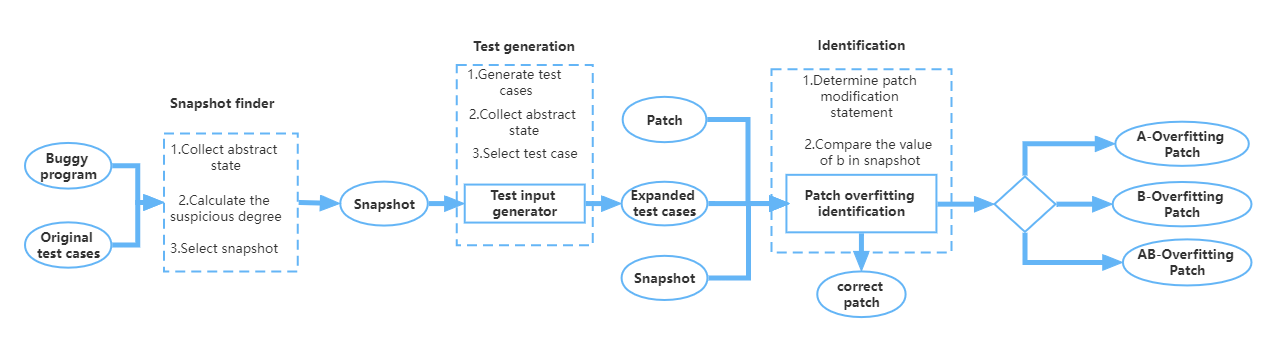
\includegraphics[width=1\textwidth]{fig5.png}
	\caption{Approach Overview}\label{fig5}
\end{figure}

Take a buggy program, an original test set $t_o$, and the corresponding patch as input. This method firstly find the most suspicious snapshot $s$ through Snapshot finder, and then generate new tests through $s$ and Test input generator. Secondly, the new tests are added to the test suite to generate the extended test suite $t_e$. PatchID runs patches with $t_e$ and saves the values of the expressions in $s$. Finally, PatchID indentifies a overfitting patch by observing whether the expression value of each test case changes before and after using the patch. And the overfitting patches are subdivided further.

\subsection{Snapshot Finder}
Snapshot finder is designed to find the most suspicious snapshot $s$. This step has two functions. One is to provide a standard for generating new tests in the next step, so as to classify the new tests; the other is to compare the snapshot set obtained after running the test set for the patch in the third step in order to identify the type of the overfitting patch.

\textbf{snapshot.} snapshot $s$ can be expressed as a 5-tuple $s= \langle \ell,b,?,i,v_i \rangle$,where $\ell$ is the unique identifier of each statement, $b$ is a boolean expression, $?$ is the value of $b$ (true or false), $i$ represents the unique serial number of each test in the test suite, and $v_i$ represents the actual value of $b$ of the test $t_i$ during $M_{bug}$ execution. Each snapshot has a corresponding degree of suspicion, which is determined by the following two factors: (1)a syntactic analysis of expression dependence $ed_s$; (2)a dynamic analysis $dy_s$. $ed_s$ increases as the number of occurrences of $b$ before and after $\ell$; The more times $?$ corresponding $b$ appears in failing tests and the less times $?$ corresponding $b$ appears in passing tests, the greater the value of $dy_s$. The formula for calculating the degree of suspicion in this paper is defined as follow:
\begin{equation}
	2/({ed_s^{-1}}+dy_s^{-1})
\end{equation}
Because of the limitation of formula above for calculating the degree of suspicion, $?$ is not exactly the same as the result $v$ of the actual execution of the test, so we must note that $?$ is used to classify new tests and $v$ is used to classify patches. Snapshot is the core of this algorithm. This paper designs the following algorithm to construct Snapshot.
\begin{algorithm}
	\caption{get the most suspicious snapshot}\label{algo1}
	\begin{algorithmic}[1]
		%\Require Input
	%\Ensure Output
	\Require
	$t_o$: original test suite;
	$M_{bug}$
	\Ensure
	 $s_{bug}$
	\State $ex_b \gets null$
	\Function {"getSnapshot"}{}
	
	\State $ex_b$ = createBooleanExpression($M_{bug}$);
	
	
	%for
	\For{each $t_i : t_o$}
	%
	
	\If {$coverBugM(t_i)$} 
	 \State $compute(ex_b)$
	\Else \State $delete(t_i)$;
	\EndIf
	\EndFor
	
	\State $s_{bug}$ = getSnapshot();
	
	\Return $s_{bug}$
	\EndFunction
	\end{algorithmic}
\end{algorithm}

In the first step of this algorithm, PatchID creates a boolean expression set for each statement $\ell$. Secondly PatchID uses $t_o$ to run the buggy program. It first deletes the tests that do not cover $M_{bug}$, then saves the program abstraction state in the tests that cover $M_{bug}$, and calculates the value of each boolean expression in the set (real value $v$). A snapshot corresponding to each coverage test is generated. The third step is to calculate the suspicious degree of each snapshot. At this time, $?$ is obtained(PatchID will use this value to generate new tests). The fourth step is to select the most suspicious snapshot $s$. If there are multiple snapshots, select one of them at random. For the subsequent process, PatchID will save a snapshot set $s_{bug}$, whose $\ell$,$b$,$?$ as with $s$, $i$ and $v$ holds the real value for each test. In the previous example, $s= \langle 3,n>=list2.size(),true,i,v \rangle$ represents the boolean expression $n>=list2.size()$ in the third line of the buggy program, the error occurs because expression is evaluated to be true.

\subsection{Test Generation}
The goal of Test generation is to generate new tests using the TEST-SIM criterion. PatchID does not need to care about whether the output of these tests is correct, but it needs to know the value of the boolean expression $b$ in the snapshot generated by these tests to be the same as $?$ of $s$. This means that PatchID requires some new failing tests that are used to enhance the test suite.

PatchID uses Evosuite\citep{bib70}, an existing automated test generation tool, to generate a set of tests. Because Evosuite generates test cases for a class, the test cases should be selected. Similar to the steps in the Snapshot finder, select the test that covers the $M_{bug}$ and save the program abstract state and snapshot. If the snapshot$(\ell,b,v)$ of the new test corresponds to the most suspicious $s(\ell,b,?)$ respectively, then new failing tests will be added to the test suite $t_e$. PatchID does not select the new passing tests, because for the passing tests, $M_{bug}$ not only outputs correctly, but also behaves correctly.

\subsection{Identification}
The purpose of this step is to determine if a patch is overfitting. It requires that snapshot set $s_{bug}$, extended test suite $t_e$, and the patch are provided previously. PatchID will run patch with the extended test suite, save the snapshot set $s_{patch}$, and then compare it with $s_{bug}$ to determine the type of patch.
\subsubsection{Select Statement}
For buggy programs, patches typically include the following operations, that is, insert, delete, replace, and update. Then the $\ell$ in the snapshot of the buggy program cannot be directly monitored in the patch, because the position of the statement has changed, and the statement $\ell_{patch}$ in the patch needs to be relocalized to monitor the same boolean expression $b$. We believe that no matter what kind of repair operation, the program can have correct program behavior only after the repair operation is completed, so the method in this paper selects the position of $\ell_{patch}$ in the next statement after the modification is completed. For some special cases, we also need to use other rules.
We denote $start_s$ as the first statement that differs between the buggy program and the patch, and $end_s$ as the last statement that differs. The rules for localizing $start_s$ and $end_s$ are defined as follows:
\begin{itemize}
	\item If $start_s$ is a block statement such as $for, while, if$, etc. and $end_s$ is inside this block statement, then $\ell_{patch}$ is the next statement at the end of the  block.
	\item If $start_s$ and $end_s$ lie in sequential statements, $\ell_{patch}$ is the next statement in $end_s$.
	\item If $end_s$ is the last statement of a program or a block of code, $\ell_{patch}$ = $end_s$
\end{itemize}
\subsubsection{Patch identification}
After $\ell_{patch}$ is determined, PatchID will run patch using the test suite $t_e$ to obtain the snapshot set $s_{patch}= \{ \langle \ell_{patch},b,?,i,v_i \rangle \mid i=0,1,\dots,n \}$. The steps for obtaining $s_{patch}$ are similar to those in 4.2. The next step is to compare two snapshot sets $s_{bug}$ and $s_{patch}$ to determine whether the patch is overfitting.
In order to identify overfitting patches, two variables $N_f$ and $N_p$ are needed to be calculated. For a failing test, $N_f$ represents the number of same value of $v$ between the two sets. For a passing test, $N_p$ represents the number of different value of $v$ between the two sets. Given the values of the variables $N_f$ and $N_p$, the type of patch is defined as follows:
\begin{equation}
	detection(p)= \begin{cases} A& N_f>0\bigwedge N_p = 0\\ B& N_f=0\bigwedge N_p>0\\
		AB& N_f>0\bigwedge N_p>0\\ correct& N_f = N_p = 0\end{cases}
\end{equation}
We map two snapshot sets one by one according to the unique identifier $i$ of the test, and compare the $v_i$ values of each test before and after using the patch. Depending on the type and source of tests, $t_e$ is divided into three categories, that is passing, failing, and new. If $t_i \in t_{passing}$, $N_p++$ when $v_i$ is different; if $t_i \in t_{failing} \cup t_{new}$, $N_f++$ when $v_i$ is the same. After the two sets are compared, the values of $N_f$ and $N_p$ can be obtained. The type of the patch can be determined according to the above formula, $N_f$ and $N_p$.
For example, $v$ corresponding to tese1 and test2 in the buggy program is false and true respectively. And both of their values in patch are false. Then $N_f = N_p = 0$, and patch is treated as correct.

\section{EVALUATION}\label{sec5}
To experimentally evaluate the effectiveness of the PatchID, we propose the following six research questions:
\begin{itemize}
	\item RQ 1: Can PatchID identify overfitting patches and classify correct patches generated by automated program repair? Does it have advantages over other methods?
	\item RQ2: How efficient is PatchID while identifing patches?
	\item RQ3: How reliable is PATCH-SIM based on boolean expressions?
	\item RQ4: What causes false positives and false negatives?
	\item RQ5: How useful is test generation for PatchID?
	\item RQ6: How reliable is PatchID for overfitting patch classification?
\end{itemize}
\subsection{Dataset}
In this paper, Patch is evaluated on two datasets. The one is the dataset collected in \citep{bib8}, which is composed of the patches generated by six APRs on Defects4J. Another is Java+JML dataset created by Nilizadeh et al.
\textbf{Defects4J.} At present, Defecets4j proposed by Just\citeyearpar{bib49} is the most widely used Java program dataset in the field of automatic program repair. Defects4J has 17 projects so far, which contain 835 defects. Each program defect in this dataset contains at least one test that can trigger it.This paper uses the six most frequently used projects in the dataset, namely, Chart, Time, Math, Lang, Closure and Mockito, where Chart is a project dedicated to displaying icons, Time is a project used for date and time processing, Math is a project for scientific computing, and Math is a project for displaying icons; Lang is a set of additional methods for manipulating JDK classes; Closure is an optimizing compiler for Javascript; Mockito is a mock framework for unit testing.The number of bugs contained in each project is shown in Table \ref{tab1} below.
\begin{table}[ht]
	\begin{center}
		\begin{minipage}{174pt}
			\caption{Defects4j Project evaluated}\label{tab1}%
			\begin{tabular}{@{}llll@{}}
				\toprule
				Project Name & Number of bugs  \\
				\midrule
				Chart    & 26   \\
				Time    & 26   \\
				Math    & 106     \\
				Lang    & 64     \\
				Closure    & 174     \\
				Mockito    & 38     \\
				Total    & 434     \\
				\botrule
			\end{tabular}
		\end{minipage}
	\end{center}
\end{table}
In this paper, six existing repair tools are used to repair the Defects4J dataset, and candidate patches are obtained. The six APRs are jGenProg, Nopol 2015, Nopol 2017, ACS, HDRepair and jKali, respectively. jGenProg is the Java version of GenProg, which is a heuristic search repair tool based on genetic algorithm. Nopol is a technique for fixing conditional statement errors in Java programs. It gives different repair strategies according to the type of error statement. If the location of the error code is a conditional statement, Nopol usually generates a repair patch to modify the original conditional statement; if the location of the error code is a non-conditional statement, it simply adds a new condition to skip the execution of the current statement. This paper includes two versions of Nopol 2015\citep{bib69} and Nopol 2017\citep{bib40}. ACS is a conditional statement synthesis tool with high precisiton, which extracts patch templates for repair based on statistical analysis. HDRepair is also a repair tool based on statistical analysis. JKali is a re-implementation of Kali on Java, which is a repair tool to remove buggy statement only.

\textbf{Java+JML dataset.} This dataset proposed by Nilizadeh is the first proven publicly available dataset for Java programs. It consists of four parts, that is correct program,  mutated wrong program, test suite, and APR-based patch. The program for this dataset has a JML specification for experimental evaluation. Java+JML dataset implements various classic algorithms and data structures, such as bubble sort, factorial, queue, and so on. They are both formally canonical small programs written in JML and, as such, can be thought of as programs with oracle. Test suites are created using an AFL-based fuzz tool, and are divided into Small and Medium based on the size of test suite. Error programs are created by injecting a single error into each Java program using PITest, a Java program mutation tool. PITest generates errors by changing the control condition, changing the assignment expression, removing the method call, and changing the return value. The APR-based repair patches are obtained using the following repair tools: ARJA-E, Cardumen, jGenProg, jKali, jMutRepair, Kali-a, and Nopol.
\subsection{Experiment Setup}
We implemented PatchID based on JAID. JAID is an automatic repair framework for generating patches for program bugs. It collects the program abstract state and uses boolean expressions as the criteria for verifying program bugs

\textbf{RQ1.} To evaluate the effectiveness of PatchID, we ran the collected patch set and saved the results of the patch identification and the values of the important variables in a file. These variables include the statement to be monitored, the expression and value of snapshot, passing test with different values, failing test with the same value, and new test.

\textbf{RQ2.} Record the running time of each patch. The time is calculated in whole minutes, and the extra seconds are rounded up and down.

\textbf{RQ3.} Manually analyze the values of $N_f$ and $N_p$ and the corresponding tests after each patch runs, and analyze the statistical information of each value.

\textbf{RQ4.} Manually analyze misclassified patches and analyze the reason why they failed.

\textbf{RQ5.} At this point, Evosuite usually finishes generating tests in about a minute and a half. Because Evosuite's strategy is to use fewer tests to cover as many paths as possible, in practice, it can typically generate 20 $\sim$ 70 tests for a class. Through the first filter, there are usually only about ten tests covering $M_{bug}$. Due to the strict screening conditions, the number of tests that meet the requirements is usually only 0 $\sim$ 3 while further screening

\textbf{RQ6.} In order to verify the effectiveness of PatchID's classification method for overfitting patches, we manually verify the specific classification of overfitting patches. Because the Defects4J patch is too complex, this paper only analyzes it in the Java+JML dataset. The human identification is based on the different warnings generated from the warning file "esc.txt" corresponding to the buggy program and the warning file "ESC\_Repaired.txt" of the patch in the dataset and the different codes between the two programs.

\subsection{Experimental Result}
\subsubsection{Result of RQ1}
\textbf{Performance on Defects4J.} A total of 220 patches are generated on the Defects4J dataset through APR tools. PatchID conducts experiments on these 220 patches to determine whether they are overfitting patches. 166 patches are run to determine whether they are overfitting patches, while the rest of the patches fail to give the final results because they exceed the set execution time limit. Except for 9 patches, 157 patches among the 166 patches, PatchID gives the results of whether they are overfitting patches. Results are shown in Table \ref{tab2}.
\begin{table}[ht]
	\begin{center}
		\begin{minipage}{\textwidth}
			\caption{The Results Identified by PatchID in Defects4j Dataset}\label{tab2}%
		
			\begin{tabular}{cccccccc}
				\toprule
				\diagbox{Project}{Tools} &Chart	&Closure	&Lang	&Math &Mockito &Time &Total \\ \hline
				Nopol  &12 &39	&10  &26 &1 &8 &96\\ 
				jKai  &5 &0	&0  &9 &0 &1 &15\\ 
				jGenprog  &6 &0	&0  &13 &0 &1 &20\\ 
				HDRepair  &0 &0	&2 &6  &0 &1 &9\\ 
				ACS  &1 &0	&4  &11 &0 &1 &17\\ 
				Total  &24 &39	&16  &65 &1 &12 &157 \\
				\bottomrule
			\end{tabular}
		
		\end{minipage}
	\end{center}
\end{table}

Table \ref{tab3} and Table \ref{tab4} show the running results of PatchID on related defect repair tools and different projects, respectively. As shown in the table, PatchID successfully filtered out 78 patches from 157 patches, including 63 overfitting patches and 15 correct patches. For 63 overfitting patches, PatchID successfully divided them into three categories, of which A-Overfitting Patches accounted for the most, reaching 50, followed by B-Overfitting Patches with 8. Number of AB-Overfitting Patches is 5.

\begin{table}[ht]
	\begin{center}
		\begin{minipage}{\textwidth}
			\caption{Performance On Different APRs}\label{tab3}%
			\begin{tabular}{cccccccc}
				\toprule
				Tool & Correct & Overfitting &Correct identified &Overfitting identified &A
				&B &AB  \\
				\midrule
				Nopol2015    &5 &20 &2(40$\%$) &10(50$\%$) &9 &0 &1   \\
				Nopol2017    &3 &68 &2(66.66$\%$) &36(52.94$\%$) &25 &8 &3   \\
				HDRepair    &4 &5 &3(75$\%$) &1(20$\%$) &1 &0 &0     \\
				ACS    &11 &6 &7(63.63$\%$) &1(16.66$\%$) &1 &0 &0     \\
				jKali    &1 &14 &0 &8(57.14$\%$) &8 &0 &0     \\
				jGenprog    &6 &14 &1(16.67$\%$) &7(50$\%$) &6 &0 &1     \\
				Total    &30 &127 &15(50$\%$) &63(49.61$\%$) &50 &8 &5     \\
				\botrule
			\end{tabular}
		\footnotetext{"Correct/overfitting identified" indicates the number of correct classifications from the "correct/overfitting" patch by PatchID.}
		\footnotetext{A = A-Overfitting Patch,B = B-Overfitting Patch,AB = AB-Overfitting Patch}
		\end{minipage}
	\end{center}
\end{table}

\begin{table}[ht]
	\begin{center}
		\begin{minipage}{\textwidth}
			\caption{Performance On Different Projects}\label{tab4}%
			\begin{tabular}{cccccccc}
				\toprule
				Tool & Correct & Overfitting &Correct identified &Overfitting identified &A
				&B &AB  \\
				\midrule
				Lang    &6 &10 &2(33.33$\%$) &3(50$\%$) &3 &0 &0   \\
				Math    &16 &49 &8(50$\%$) &22(44.90$\%$) &20 &1 &1   \\
				Chart    &3 &21 &(33.33$\%$) &12(57.14$\%$) &10 &0 &2     \\
				Time    &2 &10 &2(100$\%$) &6(60$\%$) &5 &1 &0     \\
				Closure    &2 &37 &1(50$\%$) &20(54.05$\%$) &12 &6 &2     \\
				Mockito    &1 &0 &1(100$\%$) &0 &0 &0 &0     \\
				Total    &30 &127 &15(50$\%$) &63(49.61$\%$) &50 &8 &5     \\
				\botrule
			\end{tabular}
		\end{minipage}
	\end{center}
\end{table}

\textbf{Overfitting patch.} From Table \ref{tab4}, we can find that PatchID works well on Nopol2015, Nopol2017, jKali and jGenprog (the worst accuracy  is 50$\%$), but it works poorly on ACS and HDRepair (the best accuracy is only 20$\%$). We also found that among the overfitting patches generated by these six tools, the patches that did not fix the original errors of the program were the most, and the patches that destroyed the original correct behavior of the program were relatively few. But Nopol2015 and Nopol2017 are tools that modify program conditional statements to fix bugs. A total of 12 patches destroyed the correct behavior of the program, while only jGenprog produced an AB-Overfitting Patch. We suspect that it is relatively easy to introduce new errors by modifying the conditional statements of the program.
According to Project, the accuracy of overfitting patch identification is relatively stable, ranging from 43$\%$ to 60$\%$. PatchID has the highest accuracy in Time Project, at 60$\%$. The accuracy in Math is the lowest, only 44.90$\%$. Here, the largest number of patches that destroy the original correct behavior of the program is Closure, with a total of 8.

\textbf{Correct patch.} Out of 157 patches, there are 30 correct patches, while PatchID can correctly classify 15 patches with an accuracy of 50$\%$. This is exciting messages. As far as we know, there is no tool that has such a high accuracy accuracy. Among the patches generated by Nopol2017, HDRepair and ACS, the accuracy of PatchID is more than 60$\%$, and the highest is 75$\%$. From the perspective of Project, except Lang and Chart, the accuracy of other projects is not low. Of particular note is the 100$\%$ success rate on Mockito and Time projects.

Relative to Xiong's results on this dataset, we identified one more overfitting patch than Xiong's method, but Xiong's method did not identify any correct patch, while PatchID identified 15. For 220 patches, his method identified a total of 62 and PatchID identified 78 patches. However, Xiong improved the accuracy to 56.3$\%$ by pruning the average, and the PatchID is 49.7$\%$. In addition, Xiong's method can only identify the patches of Chart, Lang, Math and Time, while PatchID involves the patches of six projects. PatchID is more extensive in its versatility.

\textbf{Performance on Java+JML dataset.} We selected 236 overfitting patches based on the Medium test suite and 336 overfitting patches based on the Small test suite from the Java+JML dataset. These overfitting patches are identified by the JML specification. In addition, there are 21 FalseNegatives patches (JML specification misidentify a correct repaired program as overfitted). The PatchID was run on a total of 593 patches, and the results of 380 patches were obtained, as shown in Table \ref{tab5}.

\begin{table}[ht]
	\begin{center}
		\begin{minipage}{175px}
			\caption{Performance On Different Projects}\label{tab5}%
			\begin{tabular}{ccc}
				\toprule
				PatchType & Collected & Validated \\
				\midrule
				Medium    &236 &144 \\
				Small    &336 &221 \\
				FalseNegatives   &21 &15 \\
				Total   &593 &380 \\
				\botrule
			\end{tabular}
		\end{minipage}
	\end{center}
\end{table}

It can be seen from the data in Table \ref{tab6} that PatchID can correctly identify 72 overfitting patches for Medium, with an accuracy of 50$\%$; PatchID can identify 92 overfitting patches for Small, with an accuracy of 41.62$\%$; In the patch of FalseNegatives, 5 correct patches were identified, and the accuracy is only 33.33$\%$.

From the perspective of overfitting classification, PatchID does not identify any B-Overfitting patches on this dataset. Moreover, except for 4 AB-Overfitting patches, all other overfitting patches are of A-Overfitting type.

From the accuracy of Medium and Small, it is clear that as the number of tests in the test suite decreases, the success rate also decreases. This data shows that weak test suites can affect the accuracy of PatchID.

\begin{table}[ht]
	\begin{center}
		\begin{minipage}{\textwidth}
			\caption{Performance On Different PatchType}\label{tab6}%
			\begin{tabular}{cccccc}
				\toprule
				PatchType & Correct identified & Overfitting identified &A &B &AB
				\\
				\midrule
				Medium    &72(50$\%$) &72(50$\%$) &72 &0 &0    \\
				Small    &129(58.37$\%$) &92(41.62$\%$) &88 &0 &4    \\
				FalseNegatives    &5(33.33$\%$) &10(66.67	$\%$) &10 &0 &0    \\
				Total    &206 &174 &170 &0 &4    \\
				\botrule
			\end{tabular}
		\end{minipage}
	\end{center}
\end{table}

\subsubsection{Result of RQ2}
\textbf{Performance on Defects4J.} We recorded the running time of 157 patches. As mentioned earlier, PatchID identifies a patch in three steps. And each step takes different amounts of time for different projects. As shown in Table \ref{tab7}, PatchID will get results in 5 minutes for most (57.32$\%$) of the patches, in which the second step of Test Generation takes up most of the time. Patches that take more than five minutes to run take more time to get the abstract state of the program, because we have observed that Evosuite typically takes 1 to 2 minutes to generate new tests on Defects4J. In the experiment, there are three patches that take more than 60 minutes to run, one of which takes 123 minutes, and most of the time is spent running tests. The average time is 11.6 minutes to identify whether a patch is overfitting, and 76.42$\%$ of the patches are within the acceptable range of t $<$ 10 min, which is satisfactory.

\begin{table}[ht]
	\begin{center}
		\begin{minipage}{\textwidth}
			\caption{Running time distribution of different projects}\label{tab7}%
			\begin{tabular}{ccccc}
				\toprule
				Project & t $<=$ 5 & t $<=$ 10 &t $<=$ 30 &t $>$ 30\\
				\midrule
				Chart	&22	&2&	0&	0\\
				Lang&	12&	2&	1&	1\\
				Math&	37&	12&	6&	10 \\
				Time&	8&	0&	3&	1\\
				Mockito&	1&	0	&0&	0\\
				Closure&	10&	14&	10&	5\\
				Total&	90(57.32$\%$)&	30(19.10$\%$)&	20(12.73$\%$)&	17(10.83$\%$)\\
				\botrule
			\end{tabular}
		\end{minipage}
	\end{center}
\end{table}

The experimental results of the memory occupied by the algorithm are shown in Figure \ref{fig6}. Among the 157 patches, 145 patches use less than 512MB of memory to obtain the results, another 10 patches use less than 1024MB of memory, and only 2 patches use more than 1024MB of memory. The patch that uses the most memory is still the one in Closure project, which uses 1405 MB of memory, and the other in Math project, which uses 1044 MB of memory.

Figure \ref{fig7} shows the average amount of memory used by each project. The  average memory used for Mockito is the least, with only 50 MB used. Others are Time, Lang, Math, Chart, Closure in descending order. The average memory used for Closure is 349MB. From our experimental data, Closure is the most time-consuming and memory-consuming, which means that our method consumes more resources in terms of Javascript optimizing compiler.

\begin{figure}[ht]%
	\centering
	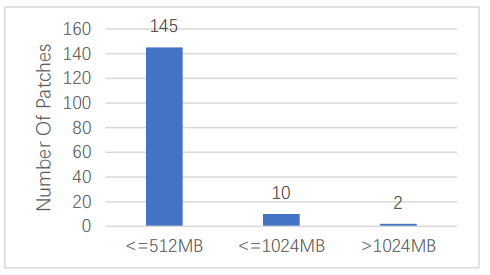
\includegraphics[width=0.5\textwidth]{fig6.png}
	\caption{Distribution of patches in memory used}\label{fig6}
\end{figure}

\begin{figure}[h]%
	\centering
	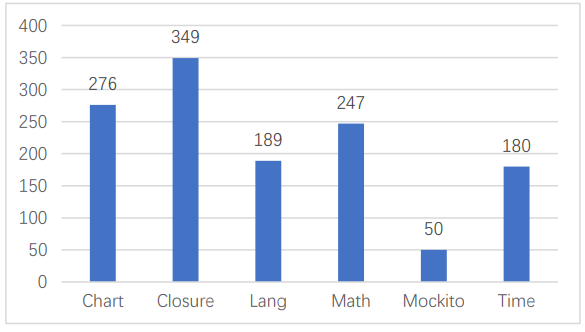
\includegraphics[width=0.5\textwidth]{fig7.png}
	\caption{Average memory used by the project}\label{fig7}
\end{figure}

\textbf{Performance on Java+JML dataset.} We recorded the distribution of the time spent of the 380 patches and the average amount of memory they used. From Table \ref{tab8}, we can see that 378 patches can produce results within 10 minutes, and only 2 patches exceed 10 minutes. From Figure \ref{fig8}, Medium patch uses the most memory, at 99 MB. The smallest is FalseNegatives, which is only 62 MB. However, none of these three types of patches exceed 100MB.

\begin{table}[ht]
	\begin{center}
		\begin{minipage}{173px}
			\caption{Number of patches at running time interval for different PatchType}\label{tab8}%
			\begin{tabular}{ccc}
				\toprule
				PatchType & t $<=$ 10 & t $>$ 10
				\\
				\midrule
				Medium    &143 &1  \\
				Small    &200 &1     \\
				FalseNegatives    &15 &0    \\
				Total    &378 &2    \\
				\botrule
			\end{tabular}
		\end{minipage}
	\end{center}
\end{table}

\begin{figure}[h]%
	\centering
	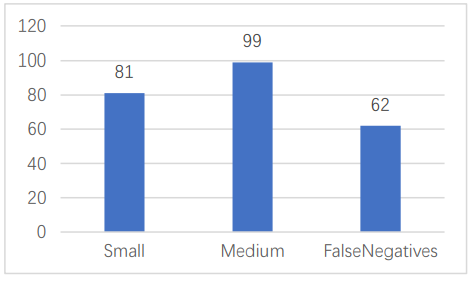
\includegraphics[width=0.5\textwidth]{fig8.png}
	\caption{Average memory used by the PatchType}\label{fig8}
\end{figure}

\subsubsection{Result of RQ3}
\textbf{Performance in Defects4J.} We observed the values of $N_f$ and $N_p$ from 63 overfitting patches, and we obtained the following two tables. It can be seen from Figure 7 that the number of patches with $N_f$ = 1 is the largest, 47. Most of the patches have $N_f$ values between 0 and 2. This shows that it is very difficult to identify a patch simply by the test output, because when the patch has only one program behavior error, its error is not reflected in the test output. PatchID, on the other hand, focuses on the behavior of the program, and as long as the wrong behavior of the program is exposed by a failed test, then the patch can be identified as overfitting.

Table \ref{tab9} shows $N_p$ values for each patch with a regression error. We find that more than half of the patches have a large $N_p$, with the maximum reaching 764. The patch note for this maximum breaks a very important correct behavior in the original program, which causes such a large number of passing tests to behave incorrectly. It is worth mentioning that from the distribution of Project, Closure still accounts for the majority of the number.

Generally speaking, PATCH-SIM works better, and it can effectively distinguish the three types of overfitting patches. And we got an interesting conclusion: on the one hand, the overfitting patch can fix the wrong behavior of the original program to some extent, but it still can not completely fix its errors; on the other hand, once the overfitting introduces the regression error, the regression error will have a greater impact on the original correct behavior of the program.

\begin{figure}[ht]%
	\centering
	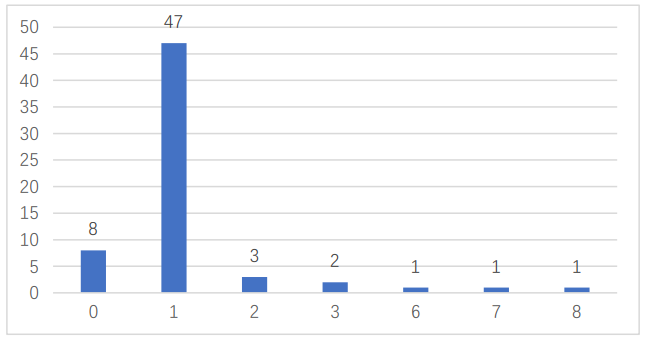
\includegraphics[width=0.5\textwidth]{fig9.png}
	\caption{Number of patches per $N_f$ value}\label{fig9}
\end{figure}

\begin{table}[ht]
	\begin{center}
		\begin{minipage}{173px}
			\caption{Patches with regression fault}\label{tab9}%
			\begin{tabular}{ccc}
				\toprule
				Patch & Project & $N_P$
				\\
				\midrule
				Patch105&	Closure&	764  \\
				Patch112&	Closure&	14     \\
				Patch119&	Closure&	19  \\
				Patch137&	Closure&	41  \\
			Patch138	&Closure&	53	\\
			Patch141&	Closure&	9	\\
			Patch147&	Closure&	1	\\
			Patch177&	Math&	1	\\
			Patch180&	Time&	14\\
		    Patch32	 &   Math&	5\\
	    	Patch4	  &  Chart&	1	\\
			Patch88	   & Chart&	1\\
			Patch94	    &Closure&	2\\
				\botrule
			\end{tabular}
		\end{minipage}
	\end{center}
\end{table}

\textbf{Performance in Java+JML dataset.} Table \ref{tab10} shows $N_f$ and $N_p$ results on the Small and Medium datasets of Java+JML dataset. It can be seen from the table that most of the patches have $N_f < = 10$, accounting for 90$\%$, because most of the patches in the above dataset are overfitting. $N_f$ and $N_p$ results of four AB-Overfitting patches is listed in Table \ref{tab11}, all of which are from the small type. From the table, we can see that their $N_p$ is not more than 2.

\begin{table}[ht]
	\begin{center}
		\begin{minipage}{173px}
			\caption{Distribution of $N_f$}\label{tab10}%
			\begin{tabular}{ccc}
				\toprule
				PatchType & $N_f<=10$ & $N_f>10$
				\\
				\midrule
				Small&	89&	3  \\
				Medium&	59&	13    \\
				\botrule
			\end{tabular}
		\end{minipage}
	\end{center}
\end{table}

\begin{table}[ht]
	\begin{center}
		\begin{minipage}{173px}
			\caption{AB-Overfitting Patch}\label{tab11}%
			\begin{tabular}{ccc}
				\toprule
				Patch&	$N_f$ &	$N_p$
				\\
				\midrule
				example240	&1&	2  \\
				example241&	1&	2   \\
				example308&	10&	1 \\
				example50&	1&	2\\
				\botrule
			\end{tabular}
		\end{minipage}
	\end{center}
\end{table}

\subsubsection{Result of RQ4}
We manually analyzed all the patches that were incorrectly identified by PatchID, and we believe that the following two points are the reasons for the wrong results.

\begin{itemize}
	\item Weak test suite
	\item Unsatisfying snapshot find strategy
\end{itemize}

These two reasons together lead to the wrong identification of PatchID. On the one hand, most of the test suites have only 1 $\sim$ 2 failing tests, and there are too few tests covering $M_{bug}$, which makes it less likely that PatchID can actually collect the correct boolean expression. On the other hand, although PatchID can generate a large number of snapshots, it can cause multiple snapshots to be equally suspicious for the first reason. The reason for the same suspicious degree is the defect of the suspicious degree formula. In addition, since only one snapshot can be selected as the criterion for the patch identification, PatchID only randomly selects one of them, and there is a considerable probability with an unrelated snapshot selected, which will also lead to the failure of the identification.

In addition, because we only selected new failing tests in the Test generation, our experiment paid more attention to whether the patch fixed the original error, but ignored whether the patch introduced new errors, although the experimental results showed that only 13 patches introduced new errors.

\subsubsection{Result of RQ5}
In terms of generating tests, we use the existing Evosuite tool to generate tests. For each patch, Evosuite takes approximately 1$\sim$2 minutes to generate tests. Because Evosuite is to cover as many paths as possible with as few tests as possible, which results in fewer new tests originally covering $M_{bug}$ that satisfy the boolean expression in the snapshot. But during the experiment, the new test has no effect on $N_f$. We looked at the program, and of course it's possible that Evosuite didn't generate a test that satisfied the snapshot. As mentioned in RQ3, we should add the passing tests in the generated tests to the test suite, which should theoretically enhance the role of Test generation.

\subsubsection{Result of RQ6}
Table \ref{tab12} shows the effect of PatchID on Java+JML dataset for overfitting patch classification. We find that the number of A-Overfitting patches and AB-Overfitting patches are similar, which shows that APR patches can actually introduce a large number of regression errors. In addition, the number of AB-D is much larger than that of AB-S, which also shows that regression errors generally occur in methods other than $M_{bug}$. According to the classification results of PatchID for overfitting patches, the number of correctly classified patches on Small and Medium datasets is 40 and 25 respectively, and All these patches are A-Overfitting patches.

It can be seen from Table \ref{tab12} that for most AB-Overfitting patches, PatchID will identify them as A-Overfitting patches, which is due to the limitations of PatchID. Because PatchID only verify the program abstract state of a single method $M_{bug}$, Most of the regression errors occur in methods other than $M_{bug}$, which is why there are so many AB-D patches. However, according to Table \ref{tab13}, PatchID is quite accurate in identifying the patches that do not fix the original errors. There are 163 patches (including A, AB-D, and AB-S) that do not fix the original errors, including 91 for Small and 72 for Medium. PatchID can identify all these patches that do not fix the original errors, with a success rate of 100$\%$.

\begin{table}[ht]
	\begin{center}
		\begin{minipage}{\textwidth}
			\caption{Classification Of Overfitting Patches}\label{tab12}%
			
			\begin{tabular}{cccccc}
				\toprule
				\diagbox{PatchType}{Overfitting} &A	&B	&AB-D	&AB-S &Total \\ \midrule
				Small&	44(40)	&1	&41&	6&	92(40)\\ 
				Medium	&25(25)&	0	&43&	4	&72(25)\\ 
				\botrule
			\end{tabular}
			
		\end{minipage}
	\end{center}
\end{table}

The number of manually identified patches of each category and the number of patches of each category correctly classified by PatchID are given in Table \ref{tab12}. The number in parentheses represents the number of patches correctly identified by PatchID. AB-D indicates the number of patches for methods where regression errors occur outside of the $M_{bug}$, and AB-S indicates the number of patches where regression errors still occur in the $M_{bug}$. For example, if the method X calls the $M_{bug}$, and the patch modifies the $M_{bug}$ to cause an error in the program behavior of the method X, then we consider this patch an AB-D Overfitting Patch.

\begin{table}[ht]
	\begin{center}
		\begin{minipage}{173px}
			\caption{Classification Of A Patches}\label{tab13}%
			
			\begin{tabular}{cc}
				\toprule
				\diagbox{PatchType}{Overfitting} &A-Patch \\ \midrule
				Small&	91(91)\\ 
				Medium	&72(72)\\ 
				\botrule
			\end{tabular}
			\footnotetext{A-Patch includes A-Overfitting patch and AB-Overfitting patch.}
		\end{minipage}
	\end{center}
\end{table}

\section{CONCLUSION}\label{sec6}
In this paper, an overfitting identification method is proposed, which combines program expression and program similar behavior, and overfitting patches are further divided into three categories. We implement the method PatchID proposed in this paper on the JAID framework. As we have seen in the experiment, the PatchID method is able to effectively filter out 78 patches from 157 patches for Defects4J dataset and 169 patches from 380 patches for Java+JML dataset. The experimental results show that we should dig deeper into the information given by the test suite, not just limited to test input and test output. Future work will focus on: (1) strengthening the scope of program monitoring to further improve the success rate of overfitting patch classification, (2) providing an effective repair scheme for the identified overfitting patches to make them closer to the correct patches.
\nocite{*}
%\bibliographystyle{spbasic}
%\bibliographystyle{plainnat}
\bibliography{manualscript}

\end{document}
